\documentclass[12pt]{article}
\usepackage{minted}
\usepackage{graphics}
\renewcommand{\baselinestretch}{1.0}

\title{\textbf{Practical Work 2}}
\author{\textbf{Group 5}}
\date{\textbf{January 2022}}

\begin{document}

\maketitle

\section{File transfer using RPC}
\hspace{0.5cm}
\vspace{0.5cm}
 Files: \mintinline{text}{serve.py}, \mintinline{text}{client.py}
 
 The practical work is implemented with Python using the library XMLRPC. It's a simple system. The client will send a file as binary data and the server will try to capture and write it down.
\vspace{0.5cm}

 First thing, we created a new server instance at port 3000 of our localhost. The server then listens for the client's signal and writes the file to paper using the function defined in the server at initialization.

\section{Design RPC}
\begin{figure}[h]
    \centering
    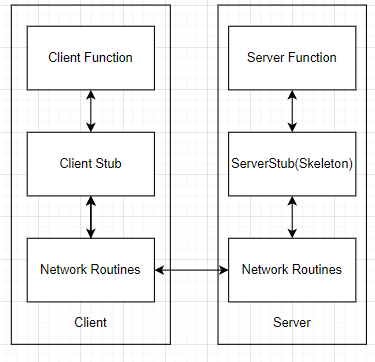
\includegraphics{image/How.png}
    \caption{RPC service}
    \label{fig:my_label}
\end{figure}
\newpage
\section{Implementation}
\subsection{Client}
\begin{minted}{python}
from aifc import Error
from xmlrpc.client import MultiCall, ServerProxy,Binary
import os
import datetime
from tkinter import Tk
from tkinter.filedialog import askopenfilename
from xmlrpc.server import XMLRPCDocGenerator

tk=Tk()
tk.withdraw()
tk.geometry('100x200')
filename=askopenfilename()
date_time_file_tranfer=os.stat(filename).st_ctime
time=datetime.date.fromtimestamp(date_time_file_tranfer)
time.strftime('%d-%m-%Y')

file=open(filename,'rb')
factory_bin=Binary(file.read())

try:
    Proxy=ServerProxy('http://localhost:3000')
    Proxy.file_transfer(factory_bin,filename,date_time_file_tranfer)
except Error as v:
    print("ERROR", v)
\end{minted}

\subsection{Server}
\begin{minted}{python}
import sys
from xmlrpc.server import SimpleXMLRPCServer
from xmlrpc.server import SimpleXMLRPCRequestHandler
import os
import time

# Restrict to a particular path.
class RequestHandler(SimpleXMLRPCRequestHandler):
    rpc_paths = ('/RPC2',)

# Create server
with SimpleXMLRPCServer(('localhost', 3000),
                        requestHandler=RequestHandler) as server:
    server.register_introspection_functions()

    # Register a function under a different name
    def file_transfer_function(datas,filename,dt):
        handle_file=open(filename.split('/')[-1],'wb')
        handle_file.write(datas.data)
        handle_file.close()
        return True
    print('Listerning on port 3000..........')
        
    server.register_function(file_transfer_function, 'file_transfer')
    try:
        server.serve_forever()
    except KeyboardInterrupt:
        print("\nKeyboard interrupt received, exiting.")
        sys.exit(0)
\end{minted}

\end{document}
